\documentclass[titlestyle=hang,11pt]{elegantbook}

\author{ddswhu \& Liam Huang}
\email{ddswhu@outlook.com}

\zhtitle{优美的 \LaTeX{} 书籍}
\zhend{模板}
\entitle{Elegant\LaTeX{} Book}
\enend{Template}
\version{3.00}
\myquote{Victory won\rq t come to us unless we go to it.}
\logo{logo.png}
\cover{cover.pdf}

%green color
   \definecolor{main1}{RGB}{0,120,2}
   \definecolor{second1}{RGB}{230,90,7}
   \definecolor{third1}{RGB}{0,160,152}
%cyan color
   \definecolor{main2}{RGB}{0,175,152}
   \definecolor{second2}{RGB}{239,126,30}
   \definecolor{third2}{RGB}{120,8,13}
%blue color
   \definecolor{main3}{RGB}{20,50,104}
   \definecolor{second3}{RGB}{180,50,131}
   \definecolor{third3}{RGB}{7,127,128}

\usepackage{makecell}
\usepackage{lipsum}
\usepackage{texnames}



\begin{document}
\maketitle
\tableofcontents
\mainmatter
\chapter{Elegant\LaTeX{} 系列模板介绍}

值此版本发行之际,我们 Elegant\LaTeX{} 项目组向大家重新介绍一下我们的工作,我们致力于打造一系列美观、优雅、简便的模板方便用户使用。Elegant\LaTeX{} 系列模板目前由 ElegantNote,ElegantBook,ElegantPaper,ElegantBeamer 组成,分别用于排版笔记,书籍,工作论文和幻灯片讲稿。这些子项目的名词是一体的,请在使用这些名词的时候不要将其断开(如 Elegant Note 是不正确的写法)。并且,Elegant\LaTeX{}  Book 指的即是 ElegantBook。

请用户在作者的主页下载最新版本,下载地址:\href{https://ddswhu.me/resource/}{https://ddswhu.me/resource/}。本文将介绍本模板的一些设置内容以及基本使用方法。如果您在使用此模板,欢迎把您使用此模板制作的成品发一份给我们,谢谢!如果您有其他问题,建议或者意见,欢迎联系我:\mailto{ddswhu@outlook.com}。


\section{ElegantBook 更新说明}
在这几年间,我们收到了很多用户的反馈,主要的问题涉及到字体安装,编码支持,定理浮动,定理跨页,交叉引用等等。我们思前想后,原先让用户安装字体以追求视觉上的美观并不完美,用户陷入了巨大的麻烦,这违背了我们的模板初衷。因此我们在新版中删除了这部分,用户无需安装任何字体。让我们来看下此次 ElegantBook 模板 3.0 更新的主要内容有:

\begin{enumerate}[noitemsep]
   \item 使用 \texttt{tcolorbox} 宏包改写了原先的定理类环境,目前定理环境等均可以跨页。
   \item 重新命名了定理类环境的名称(theorem,definition,proposition 等)。
   \item 重新命名了颜色的名字(first,second,third)。
   \item 删除了自定义字体设置,改用 \texttt{ctex} 宏包用以支持中文。
\end{enumerate}

\section{未来更新计划}

\begin{enumerate}[noitemsep]
   \item 设计一个适合的 LOGO;
   \item 重新设计 base 图标;
   \item 重新设计一个好看的封面。
   \item 将基础模板改为英文模板,添加选项使其支持中文。
   \item 将最早的 ElegantNote 重新设计为简版发布。
   \item 添加一个简化风格(plain)的颜色主题。
\end{enumerate}

\chapter{ElegantBook 设置说明}


\section{编译方式}

本模板基于基础的 book 文类,所以 book 的选项对于本模板也是有效的。默认编码为 UTF-8,推荐使用 \TeX{} Live 编译。作者编写环境为 Win10(64bit) + \TeX{} Live 2018。由于使用的是 \texttt{ctex} 宏包,所以支持 \texttt{pdflatex} 以及 \texttt{xelatex} 编译。


\section{选项设置}
本文特殊选项设置共有 2 类,分为 {\color{main}主题颜色}设置 以及 {\color{main}章标题显示风格}设置。

第 1 类为{\color{main}主题颜色}设置,内置 3 组颜色主题,分别为 \verb|green|(默认),\verb|cyan|,\verb|blue|,另外还有一个自定义的选项 \verb|nocolor|,用户\textbf{必须}在使用模板的时候选择某个颜色主题或选择 \verb|nocolor| 选项。调用颜色主题 \verb|green| 的方法为 \verb|\documentclass[green]{elegantbook}|或者使用 \verb|\documentclass[color=green]{elegantbook}|。需要改变颜色的话请选择 \verb|nocolor| 选项或者使用 \verb|color=none|,然后在导言区定义 main、second、third 颜色,具体的方法如下:
\begin{verbatim}
\definecolor{main}{RGB}{70,70,70}    %定义 main 颜色值
\definecolor{second}{RGB}{115,45,2}    %定义 second 颜色值
\definecolor{third}{RGB}{0,80,80}     %定义 third 颜色值
\end{verbatim}

\begin{table}[htp]
\centering
\begin{tabular}{ccccc}
\toprule
	  & green & cyan & blue & 主要使用的环境\\
\midrule
main & \makecell{{\color{main1}\rule{1cm}{1cm}}}& \makecell{{\color{main2}\rule{1cm}{1cm}}}&\makecell{ {\color{main3}\rule{1cm}{1cm}}}& definition \\

second &\makecell{ {\color{second1}\rule{1cm}{1cm}}}& \makecell{{\color{second2}\rule{1cm}{1cm}}}&\makecell{ {\color{second3}\rule{1cm}{1cm}}}&theorem \ lemma \ corollary\\

third &\makecell{ {\color{third1}\rule{1cm}{1cm}}}& \makecell{{\color{third2}\rule{1cm}{1cm}}}&\makecell{ {\color{third3}\rule{1cm}{1cm}}}&proposition\\
\bottomrule
\end{tabular}
\caption{ElegantBook 模板中的三套颜色主题\label{tab:color thm}}
\end{table}

第 2 类为{\color{main} 章标题显示风格},包含 \verb|hang|(默认)与 \verb|display| 两种风格,区别在于章标题单行显示(\verb|hang|)与双行显示(\verb|display|),本说明使用了 \verb|hang|。调用方式为 \verb|\documentclass[hang]{elegantbook}| 或者 \verb|\documentclass[titlestyle=hang]{elegantbook}|。

综合起来,同时调用三个选项使用 \verb|\documentclass[color=X,titlestyle=Y]{elegantbook}|。其中 \verb|X| 可以选择 \verb|green|,\verb|cyan|,\verb|blue|,\verb|none|;\verb|Z| 可以选择 \verb|hang| 或者 \verb|display|。

\section{数学环境简介}

在我们这个模板中,定义了三大类环境

\begin{enumerate}[noitemsep]
\item 定理类环境,包含标题和内容两部分。根据格式的不同分为3种
   \begin{itemize}[noitemsep]
      \item {\color{main}\bfseries definition} 环境,含有一个可选项,编号以章节为单位,颜色为 {\color{main}main};
      \item {\color{second}\bfseries theorem、lemma、corollary} 环境,颜色为主颜色 {\color{second}second},编号均以章节为单位;
      \item {\color{third}\bfseries proposition} 环境,含有一个可选项,编号以章节为单位,颜色为 {\color{third}{third}}。
   \end{itemize}
\item 示例类环境,有 \textbf{example、exercise} 环境,自动编号,编号以章节为单位。
\item 证明类环境,有 \textbf{proof、note} 环境,特点是,有引导符或者结尾符,\textbf{note} 环境有引导符号,\textbf{proof} 环境有证明完毕标志。
\item 结论类环境,有\textbf{conclusion、assumption、property,remark、solution} 环境,三者均以粗体的引导词为开头,和普通段落格式一致。
\end{enumerate}

\section{可编辑的字段}
在模板中,可以编辑的字段分别为作者 \verb|\author|、邮箱 \verb|\email|、中文标题 \verb|\zhtitle|、中文标题结尾 \verb|\zhend|、英文标题\verb| \entitle|、英文标题结尾 \verb|\enend|、名言 \verb|\myquote|、版本号 \verb|\version|。并且,可以根据自己的喜好把封面水印效果的 \verb|cover.pdf| 替换掉,以及封面中用到的 \verb|logo.png|。

\chapter{ElegantBook 写作示例}

\section{Economics and Differentiable Function}

Economics focuses on the behaviour and interactions of economic agents and how economies work. Microeconomics analyzes basic elements in the economy, including individual agents and markets, their interactions, and the outcomes of interactions. Individual agents may include, for example, households, firms, buyers, and sellers. Macroeconomics analyzes the entire economy (meaning aggregated production, consumption, savings, and investment) and issues affecting it, including unemployment of resources (labour, capital, and land), inflation, economic growth, and the public policies that address these issues (monetary, fiscal, and other policies). See glossary of economics.
\begin{align*}
   &\max(\min)\quad \mathbb{E}\int_{t_0}^{t_1}f(t,x,u)\,dt\\
   &\quad\mbox{s.t.} \quad dx=g(t,x,u)dt+\sigma(t,x,u)dz\\
   &\quad \hspace{2.em} k(0)=k_0\;\text{given}
\end{align*}

where $z$ is stochastic process or white noise or wiener process.

Other broad distinctions within economics include those between positive economics, describing "what is", and normative economics, advocating "what ought to be"; between economic theory and applied economics; between rational and behavioural economics; and between mainstream economics and heterodox economics.

Economic analysis can be applied throughout society, in business, finance, health care, and government. Economic analysis is sometimes also applied to such diverse subjects as crime, education, the family, law, politics, religion, social institutions, war, science, and the environment.

\begin{definition}{Differenzierbarkeit}{diff}
Eine Funktion $f:~I\to\mathbb{R}$ auf einem Intervall $I$ hei\ss{}t in $x_0\in I$ differenzierbar oder linear approximierbar, wenn der Grenzwert
   \begin{equation*}
      \lim\limits_{x\to x_0}\frac{f(x)-f(x_0)}{x-x_0}=
      \lim\limits_{h\to 0}\frac{f(x_0+h)-f(x_0)}{h}
   \end{equation*}
existiert. Bei Existenz hei\ss{}t dieser Grenzwert Ableitung oder Differentialquotient von $f$ in $x_0$ und man schreibt f\"{u}r ihn
   \begin{equation*}
      f'(x_0)\quad\text{oder}\quad\frac{df}{dx}(x_0).
   \end{equation*}
\end{definition}

The discipline was renamed in the late 19th century, primarily due to Alfred Marshall, from "political economy" to "economics" as a shorter term for "economic science". At that time, it became more open to rigorous thinking and made increased use of mathematics, which helped support efforts to have it accepted as a science and as a separate discipline outside of political science and other social sciences.

\begin{example}
$E$ and $F$ be two events such that $P(E)=
P(F)=1/2$, and $P(E\cap F)=1/3$, let $\mathscr{F}=\sigma(Y)$,  $X$ and $Y$ be the indicate function of $E$ and $F$ respectively. How to compute $\mathbb{E}[ X\mid \mathscr{F} ]$?
\end{example}

Some subsequent comments criticized the definition as overly broad in failing to limit its subject matter to analysis of markets. From the 1960s, however, such comments abated as the economic theory of maximizing behaviour and rational-choice modelling expanded the domain of the subject to areas previously treated in other fields. There are other criticisms as well, such as in scarcity not accounting for the macroeconomics of high unemployment.

\begin{exercise}
let $S=l^\infty=\big\{(x_n)\mid \exists\, M \text{ such that } \forall n, |x_n|\leq M,x_n\in \mathbb{R}\big\}$, $\rho_{\infty}(x,y)=\sup\limits_{n\geq 1}|x_n-y_n|$, show that $\big(l^\infty,\rho_{\infty}\big)$ is complete.
\end{exercise}

\begin{theorem}{Mittelwertsatz f\"{u}r $n$ Variable}{31}
Es sei $n\in\mathbb{N}$, $D\subseteq\mathbb{R}^n$ eine offene Menge und $f\in C^{1}(D,\mathbb{R})$. Dann gibt es auf jeder Strecke $[x_0,x]\subset D$ einen Punkt $\xi\in[x_0,x]$, so dass gilt
\begin{equation*}
   f(x)-f(x_0) = \operatorname{grad} f(\xi)^{\top}(x-x_0)
\end{equation*}
\end{theorem}

\begin{note}
在本模板中,引理(lemma),推论(corollary )的样式和定理的样式一致,包括颜色,仅仅只有计数器的设置不一样。
\end{note}


Gary Becker, a contributor to the expansion of economics into new areas, describes the approach he favours as "combin[ing the] assumptions of maximizing behaviour, stable preferences, and market equilibrium, used relentlessly and unflinchingly."One commentary characterizes the remark as making economics an approach rather than a subject matter but with great specificity as to the "choice process and the type of social interaction that [such] analysis involves." 


Economic efficiency measures how well a system generates desired output with a given set of inputs and available technology. Efficiency is improved if more output is generated without changing inputs, or in other words, the amount of "waste" is reduced. A widely accepted general standard is Pareto efficiency, which is reached when no further change can make someone better off without making someone else worse off.

\begin{proposition}{最优性原理}{max}
如果 $u^*$ 在 $[s,T]$ 上为最优解,则 $u^*$在$[s,T]$ 任意子区间都是最优解,假设区间为 $[t_0,t_1]$ 的最优解为 $u^*$ ,则 $u(t_0)=u^{*}(t_0)$,即初始条件必须还是在 $u^*$ 上。
\end{proposition}

Microeconomics examines how entities, forming a market structure, interact within a market to create a market system. These entities include private and public players with various classifications, typically operating under scarcity of tradable units and light government regulation. The item traded may be a tangible product such as apples or a service such as repair services, legal counsel, or entertainment.

\begin{corollary}{}{}
假设 $V(\cdot,\cdot)$ 为值函数,则根据最大值原理~\ref{thm:31},有如下推论
\[
V(k,z)=\max\Big\{u\big(zf(k)-y\big)+\beta \mathbb{E}V(y,z^\prime)\Big\}
\]
\end{corollary}

\begin{proof}
因为 $y^*=\alpha\beta z k^\alpha$,$V(k,z)=\alpha/1-\alpha\beta\ln k_0+1/1-\alpha\beta \ln z_0+\Delta$。
   \begin{align*}
   \text{右边}&=\Big\{u\big(zf(k)-y\big)+\beta \mathbb{E}V(y,z^\prime)\Big\}\\
   &=\ln(zk^\alpha-\alpha\beta zk^\alpha)+\beta\mathbb{E}\Big[\frac{\alpha}{1-\alpha\beta}\ln y+\frac{1}{1-\alpha\beta}\ln z^\prime+\Delta\Big]\\
   &=\ln(1-\alpha\beta)zk^\alpha+\beta\Big\{\mathbb{E}\big[\frac{\alpha}{1-\alpha\beta}\ln \alpha\beta z k^\alpha\big]+\frac{1}{1-\alpha\beta}\mathbb{E}[\ln z^\prime]+\Delta\Big\}
   \end{align*}
利用 $\mathbb{E}[\ln z^\prime]=0$,并将对数展开得
   \begin{align*}
   \text{右边}&=\ln (1-\alpha\beta)+\ln z+\alpha\ln k+\frac{\alpha\beta}{1-\alpha\beta}\big[\ln \alpha\beta+\ln z+\alpha\ln k\big]+\frac{\beta}{1-\alpha\beta}\mu+\beta \Delta\\
   &=\frac{\alpha}{1-\alpha\beta}\ln k+\frac{1}{1-\alpha\beta}\ln z+\Delta
   \end{align*}
所以 $\text{左边}=\text{右边}$,证毕。
\end{proof}



\begin{property}
Properties of Cauchy Sequence
\begin{enumerate}[noitemsep]
\item $\{x_k\}$ is cauchy sequence then $\{x_k^i\}$ is cauchy sequence.
\item $x_k\in \mathbb{R}^n$, $\rho(x,y)$ is Euclidean, then cauchy is equivalent to convergent, $(\mathbb{R}^n,\rho)$ metric space is complete.
\end{enumerate}
\end{property}

\begin{note}
conclusion、assumption、property,remark、solution 的环境效果是一样的。
\end{note}

Various market structures exist. In perfectly competitive markets, no participants are large enough to have the market power to set the price of a homogeneous product. In other words, every participant is a "price taker" as no participant influences the price of a product. In the real world, markets often experience imperfect competition.

Scarcity is represented in the figure by people being willing but unable in the aggregate to consume beyond the PPF (such as at $X$) and by the negative slope of the curve.[32] If production of one good increases along the curve, production of the other good decreases, an inverse relationship. This is because increasing output of one good requires transferring inputs to it from production of the other good, decreasing the latter.

\begin{figure}[!htbp]
	\centering
	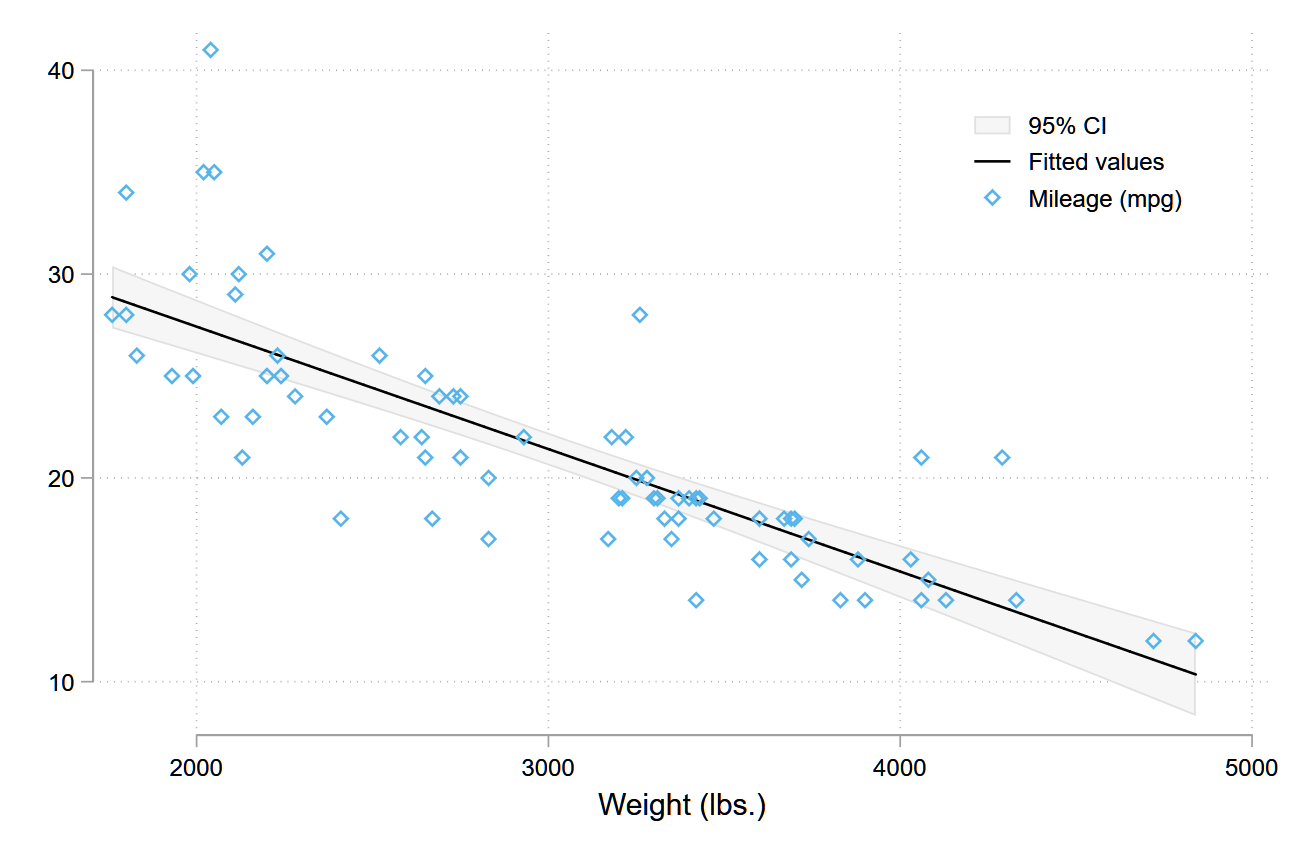
\includegraphics[width=0.6\textwidth]{mpg.png}
	\caption{The Relationship between MPG and Weight\label{fig:mpg}}
\end{figure}

\begin{definition}{Contraction mapping}{mapping}
$(S,\rho)$ is the metric space, $T: S\to S$, If there exists $\alpha\in(0,1)$ such that for any $x$ and $y\in S$, the distance
\begin{equation}
\rho(Tx,Ty)\leq \alpha\rho(x,y)
\end{equation}
Then $T$ is a {\color{main} contraction mapping}.
\end{definition}

\begin{remark}
\begin{enumerate}[noitemsep]
\item $T:S\to S$, where $S$ is a metric space, if  for any $x,y\in S$, $\rho(Tx,Ty)<\rho(x,y)$ is not contraction mapping.
\item Contraction mapping is continuous map.
\end{enumerate}
\end{remark}


\begin{conclusion}
In theory, in a free market the aggregates (sum of) of quantity demanded by buyers and quantity supplied by sellers may reach economic equilibrium over time in reaction to price changes; in practice, various issues may prevent equilibrium, and any equilibrium reached may not necessarily be morally equitable. For example, if the supply of healthcare services is limited by external factors, the equilibrium price may be unaffordable for many who desire it but cannot pay for it.
\end{conclusion}

\section{Bibliography}
This template uses Bib\TeX{} to generate the bibliography, the default bibliography style is \verb|aer|. ~\cite{Chen2018} use data from a major peer-to-peer lending marketplace in China to study whether female and male investors evaluate loan performance differently. You can add bib items (from Google Scholar, Mendeley, EndNote, and etc.) to \verb|reference.bib| file, and cite the bibkey in the \verb|tex| file.


\nocite{EINAV2010,Havrylchyk2018} 

\bibliographystyle{aer}
\bibliography{reference}

\addcontentsline{toc}{chapter}{参考文献}

\end{document}
